%%%%%%%%%%%%%%%%%%%%%%%%%%%%%%%%%%%%%%%%%
% Focus Beamer Presentation
% LaTeX Template
% Version 1.0 (8/8/18)
%
% This template has been downloaded from:
% http://www.LaTeXTemplates.com
%
% Original author:
% Pasquale Africa (https://github.com/elauksap/focus-beamertheme) with modifications by 
% Vel (vel@LaTeXTemplates.com)
%
% Template license:
% GNU GPL v3.0 License
%
% Important note:
% The bibliography/references need to be compiled with bibtex.
%
%%%%%%%%%%%%%%%%%%%%%%%%%%%%%%%%%%%%%%%%%

%----------------------------------------------------------------------------------------
%	PACKAGES AND OTHER DOCUMENT CONFIGURATIONS
%----------------------------------------------------------------------------------------

\documentclass{beamer}
%\documentclass[handout]{beamer}


\def\documentauthorname         {Рафаел Калъчев}

\def\documentauthoremail        {kalachev.rafael@gmail.com}

\def\documenttitle              {Платформа за безпилотен летателен апарат с четири ротора}

\def\documentsubject            {Автоматика}

\def\documentkeywords           {математика,автоматика,управление}

\def\documenttype               {Дипломна работа}

\def\documentlocation           {Технически университет - София}


\usepackage{fontspec}
\usepackage{microtype}
\setmainfont[Ligatures={TeX,Common,Rare}]{Heuristica}

\newfontfamily{\cyrillicfonttt}{Heuristica}
\newfontfamily{\cyrillicfontsf}{Heuristica}
\newfontfamily{\englishfonttt}{Fira Code}


\usepackage{graphicx}
\usepackage{scalerel}
\graphicspath{
    {graphics/}
    {src/}
}


\usepackage{polyglossia}
\setdefaultlanguage{bulgarian}

\captionsbulgarian{
  \def\equationname{Уравнение}%
  \def\footnotename{Бележка}%
  \def\itemname{Точка}%
  \def\figurename{Фигура}%
  \def\tablename{Таблица}%
  \def\partname{Част}%
  \def\appendixname{Апендикс}%
  \def\chaptername{Глава}%
  \def\sectionname{Секция}%
  \def\subsectionname{Събсекция}%
  \def\subsubsectionname{Събсъбсекция}%
  \def\paragraphname{Параграф}%
  \def\subparagraphname{Събпарагра}%
  \def\FancyVerbLinename{Линия}%
  \def\theoremname{Теорема}%
  \def\pagename{Страница}%
}

\makeatletter
\ifdefined\HyLang@bulgarian\else
\gappto\blockextras@bulgarian{%
  \def\equationautorefname{Уравнение}%
  \def\footnoteautorefname{Бележка}%
  \def\itemautorefname{Точка}%
  \def\figureautorefname{Фигура}%
  \def\tableautorefname{Таблица}%
  \def\partautorefname{Част}%
  \def\appendixautorefname{Апендикс}%
  \def\chapterautorefname{Глава}%
  \def\sectionautorefname{Секция}%
  \def\subsectionautorefname{Събсекция}%
  \def\subsubsectionautorefname{Събсъбсекция}%
  \def\paragraphautorefname{Параграф}%
  \def\subparagraphautorefname{Събпарагра}%
  \def\FancyVerbLineautorefname{Линия}%
  \def\theoremautorefname{Теорема}%
  \def\pageautorefname{Страница}%
}
\let\inlineextras@bulgarian\blockextras@bulgarian
\fi

\ifdefined\HyLang@english\else
\appto\blockextras@english{%
  \def\equationautorefname{Equation}%
  \def\footnoteautorefname{footnote}%
  \def\itemautorefname{item}%
  \def\figureautorefname{Figure}%
  \def\tableautorefname{Table}%
  \def\partautorefname{Part}%
  \def\appendixautorefname{Appendix}%
  \def\chapterautorefname{Chapter}%
  \def\sectionautorefname{section}%
  \def\subsectionautorefname{subsection}%
  \def\subsubsectionautorefname{subsubsection}%
  \def\paragraphautorefname{paragraph}%
  \def\subparagraphautorefname{subparagraph}%
  \def\FancyVerbLineautorefname{line}%
  \def\theoremautorefname{Тheorem}%
  \def\pageautorefname{page}%
}
% \inlineextras@english is empty, so we simply set it
% equal to \blockextras@english
\let\inlineextras@english\blockextras@english
\fi
\makeatother


\setotherlanguage{english}
\usepackage{verbatim}

\usetheme{focus} % Use the Focus theme supplied with the template
% Add option [numbering=none] to disable the footer progress bar
% Add option [numbering=fullbar] to show the footer progress bar as always full with a slide count

% Uncomment to enable the ice-blue theme
%\definecolor{main}{RGB}{92, 138, 168}
%\definecolor{background}{RGB}{240, 247, 255}

%------------------------------------------------

\usepackage{booktabs} % Required for better table rules

%----------------------------------------------------------------------------------------
%	 TITLE SLIDE
%----------------------------------------------------------------------------------------
\makeatletter
\@ifpackageloaded{babel}
  {\newenvironment{nohyphens}
     {\par\sloppy\exhyphenpenalty=\@M
      \@ifundefined{l@nohyphenation}
        {\language=\@cclv}
        {\hyphenrules{nohyphenation}}%
     }
     {\par
      \@ifundefined{l@nohyphenation}
        {}
        {\endhyphenrules}%
     }
  }
  {\newenvironment{nohyphens}
     {\par\sloppy\exhyphenpenalty=\@M
      \@ifundefined{l@nohyphenation}
        {\language=\@cclv}
        {\language=\l@nohyphenation}%
     }
     {\par}
  }
\makeatother

\title{\documenttitle}


\subtitle{}

\author{\documentauthorname}

\titlegraphic{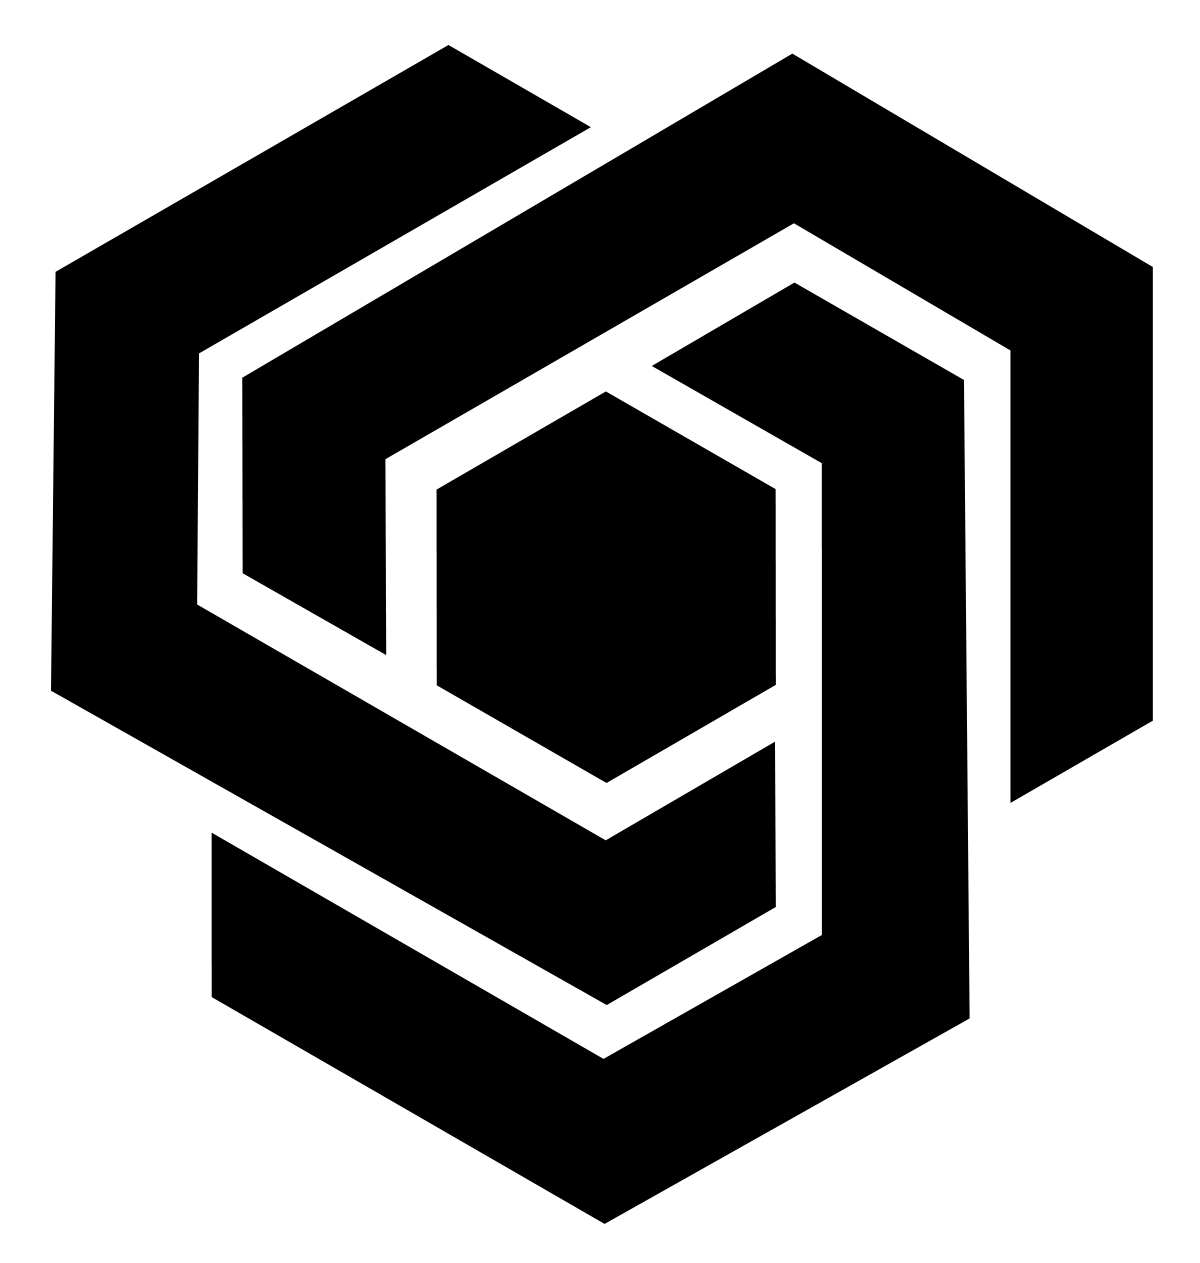
\includegraphics[width=0.2\textwidth]{Images/logo.png}} % Optional title page image, comment this line to remove it

\institute{Технически Университет София}

\date{25 Февруари 2022}

%------------------------------------------------
%\setlength{\parskip}{1.5em}
\linespread{1.25}



\begin{document}

%------------------------------------------------
	
\begin{frame}
	\begin{nohyphens}
	\maketitle % Automatically created using the information in the commands above
	\end{nohyphens}
\end{frame}

%----------------------------------------------------------------------------------------
%	 SECTION 1
%----------------------------------------------------------------------------------------

\section{Увод} 

\subsection{Цели и задачи - Софтуер}


\begin{frame}{Цели и задачи - Софтуер}
	\begin{itemize}
		\pause 
		\item Изграждане на среда за разработка на софтуер с основа \textit{Make} под \textit{Linux}

		\pause 
		\item Подбор на хардуерни и софтуерни решения за интеграция с разработената среда

		\pause 
		\item Създаване на софтуерни модули и драйвъри за работа с вътрешния и външен хардуер

		\pause 
		\item Подбор на изходни портове, пинове и нужна периферия

		\pause
		\item Инициализация и конфигурация на микроконтролера и периферията 

	\end{itemize}
\end{frame}

\subsection{Цели и задачи - Хардуер}


\begin{frame}{Цели и задачи - Хардуер}
	\begin{itemize}
		\pause 
		\item Разположение на хардуера и избор на конфигурация за системата 

		\pause 
		\item Подбор на изходни портове, пинове и нужна периферия

		\pause
		\item Свързване на компонентите и електроснабдяване

		\pause 
		\item Изграждане платформи за опитни постановки

		\pause 
		\item Сглобаване на системата

	\end{itemize}
\end{frame}

\subsection{Цели и задачи - Идентификация,\\ моделиране, наблюдение и управление}


\begin{frame}{Цели и задачи -  Идентификация,\\ моделиране, наблюдение и управление }
	\begin{itemize}
		\pause 
		\item Моделиране:

		\begin{itemize}
			\pause 
			\item Ротор с витло

			\pause 
			\item Платформа за управление на ъгъл на завъртане

			\pause 
			\item Платформа за безпилотен летателен апарат с четири ротора

		\end{itemize}
		\pause 
		\item Идентификация на параметри

		\pause 
		\item Компенсация на сензорни отмествания

		\pause
		\item Калибриране на сензорите

		\pause
		\item Синтез на наблюдател за оценка на ориентацията на платформата

		\pause 
		\item Синтез на управление
	\end{itemize}
\end{frame}


%------------------------------------------------

\section{Софтуерна част}

\subsection{Среда за разработка на софтуер с основа\\\textit{Make} под \textit{Linux}}


\begin{frame}{Описание и съставни части}
	\begin{columns}
		\column{0.7\textwidth}
		\begin{block}{ Състав на средата за работа под \textit{Linux}}
			\begin{itemize}
				\pause
				\item Система за насочено изграждане: \\ \textit{GNU Make}

				\pause
				\item \textbf{Kомпилатор:} \\ \textit{GCC ARM NON-EABI}

				\pause
				\item \textbf{Връзка с контролера:} \\ \textit{ST-LINK}

				\pause
				\item \textbf{Текстов редактор:} \\\textit{VIM + Ctags}

				\pause 
				\item \textbf{Дебъгер:} \\ \textit{GDB (GNU Project Debuger)} 

			\end{itemize}
		\end{block}
		\column{0.15\textwidth}
		\pause
			
\includegraphics[width=0.95\linewidth]{Images/make.png} \\[0.5em]
			
\includegraphics[width=0.95\linewidth]{Images/gcc.png}
		\column{0.15\textwidth}
			
\includegraphics[width=0.95\linewidth]{Images/st-link.png} \\[0.5em]
			
\includegraphics[width=0.95\linewidth]{Images/vim.png}\\[0.5em]
			
\includegraphics[width=0.95\linewidth]{Images/gdb.png}
	\end{columns}
\end{frame}

\begin{frame}{Команден итерфейс}

	\begin{block}{Подържани команди }
	\begin{description}
		\pause
		\item[make | make all] Цялостно изграждане чрез компилиране и свързване на всчики \emph{нужни} елементи.

		\pause
		\item[make clean] Изчистване на средата.

		\pause
		\item[make flash] Запис на изградения
		\footnote{В случай, че софтуерът има нужда от (пре)изграждане, системата автоматично го (пре)изгражда.}
		софтуер в паметта на микроконтролера.

	\end{description}
	\end{block}
\end{frame}

\begin{frame}[t]
	\begin{block}{ }
	\begin{description}
		\pause
		\item[make debug] Отваряне на порт за дебъг, стартиране и свързване на дебъгера
		\footnote{Системата автоматино конфигурира дебъгера да използва дебъг символите в изградения софтуер.}

		\pause
		\item[make usart] Стартира интерактивен комуникационен интерфейс за връзка (IO) с контролера чрез USART.

		\pause
		\item[make usart\_read] Създава файл, съдържащ получените данни през USART порта.

	\end{description}
	\end{block}
\end{frame}


\begin{frame}{Подбрани хардуерни и софтуерни решения за анализ}
	\begin{columns}
		\column{0.7\textwidth}
		\pause
		\begin{block}{ }
			\begin{itemize}
				\pause
				\item Логически анализатор и генератор на логически сигнали
					\begin{itemize}
						\pause
						\item SQ50 - logic analyzer (IKALOGIC S.A.S)
						\pause
						\item ScanaStudio 16.04 (for Linux)
					\end{itemize}
				\pause
				\item UART / USB Конвертор + picocom
			\end{itemize}
		\end{block}
		\column{0.3\textwidth}
		\pause
		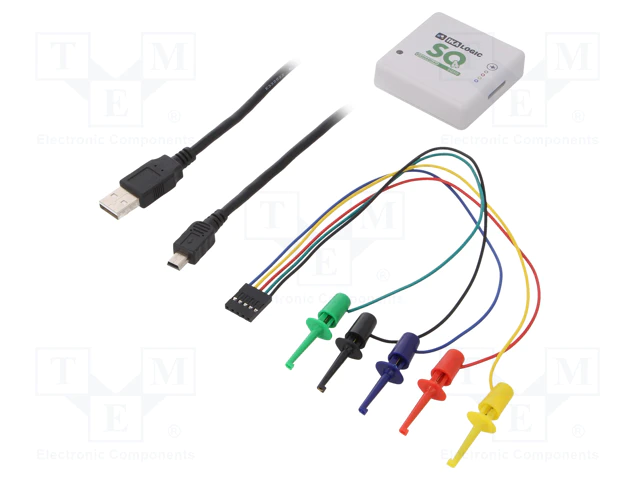
\includegraphics[width=0.8\linewidth]{Images/SQ50-logic-analyzer.png} \\[0.5em]
		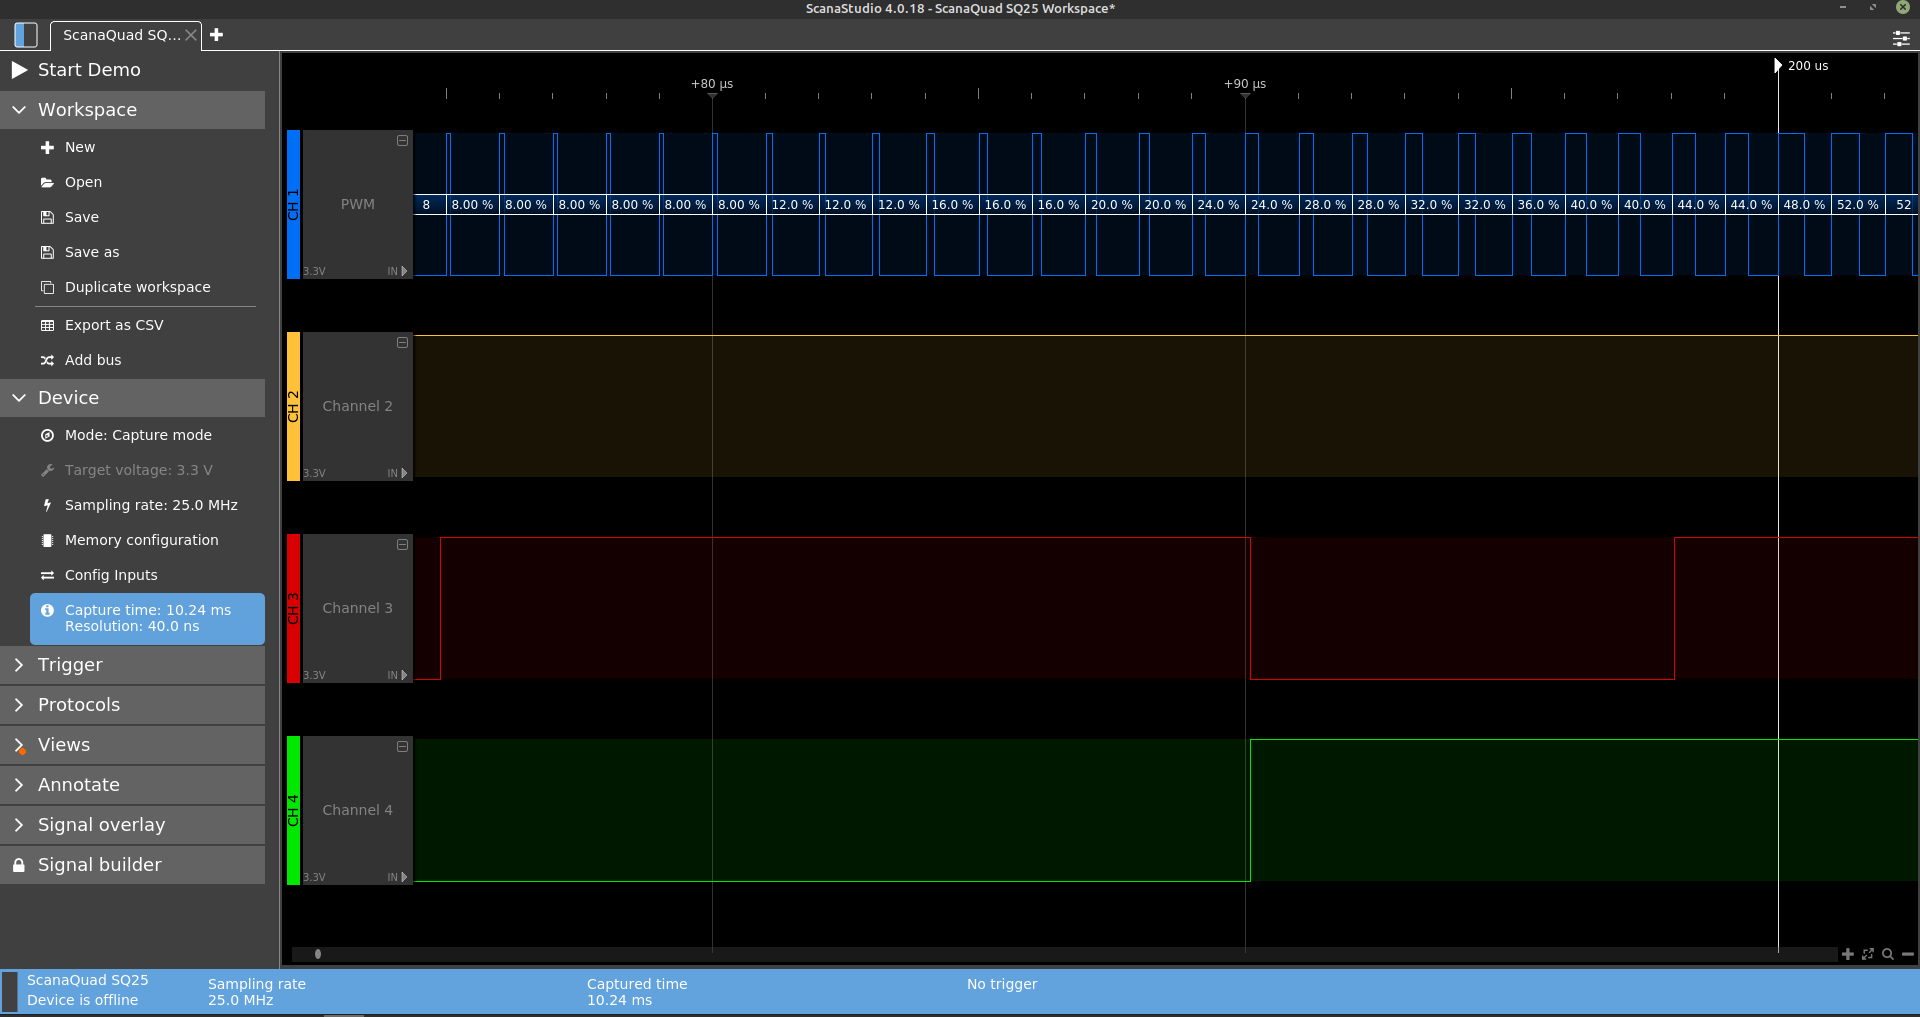
\includegraphics[width=0.8\linewidth]{Images/scana_studio_window.png}\\[0.5em]	
		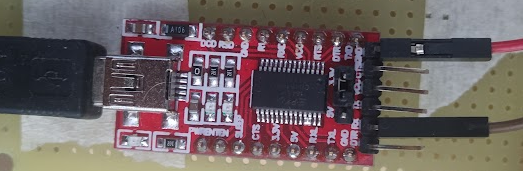
\includegraphics[width=0.9\linewidth]{Images/uart_usb.png} \\[0.5em]
	\end{columns}
\end{frame}


\begin{frame}{Решени задачи по отнощение на средата}
	\pause
		\begin{block}{Конфигурация на компилатор}
			\begin{itemize}
				\pause
				\item Използване на хардуерния модул за числа с плаваща запетая
				\pause
				\item Изключване на оптимизациите
				\pause
				\item Генериране на символи за дебъг
			\end{itemize}
		\end{block}
\end{frame}

\begin{frame}[t]
	\pause
		\begin{block}{Линкерен скрипт}
			\begin{itemize}
				\pause
				\item Очертаване на разположението на отделните секции в паметта
				\pause
				\item Генериране на символи, използвани от буутлоудъра.
				\pause
				\item Правилно подравняване на отделните секции.
				\pause
				\item Остранване на символи от стнадартните библиотеки.
			\end{itemize}
		\end{block}

		\pause

	\begin{block}{Конфигурация на дебъгер}
		\begin{itemize}
			\pause
			\item Автоматично отваряне на сесия и подвързване към дебъгерният порт.
			\pause
			\item Предварително зареждане на дебъг символите от последния обектен файл.
		\end{itemize}
	\end{block}

\end{frame}


\subsection{Софтуерни модули за вътрешна и външна\\периферия}

\begin{frame}{Описание на модулите за вътрешна\\периферия}
	\pause
	Софтуерните модули са изградени на база описанието на регистирте за вътрешната периферия, посочени в 
	документа за техническа справка на микроконтролери от семейство \textit{STM32F4xxx} \cite{stmcurefman}.\\[1.5em]

	\pause
	Основите за регистърните блокове на периферията в паметта са описани в дкоумента за съответния
	модел микроконтролер \cite{stmmcudatasheet}.

\end{frame}

\begin{frame}{Изградени модули за вътрешна периферия}
	\pause
	\begin{block}{RCC (Reset and Clock Control)}
		\pause
		Модул за управление на:
		\begin{itemize}
			\pause
			\item Времеви бази (clock source: HSE, HSI, LSE)
			\pause
			\item PLL честотен множител
			\pause
			\item Делители на честота
			\pause
			\item Часовници на периферните шини
			\pause
			\item Часовници на периферията
		\end{itemize}
	\end{block}

\end{frame}

\begin{frame}[t]
	\pause
	\begin{block}{NVIC (Nested Vectored Interrupt Controller)}
		\pause
		Модул за управление на:
		\begin{itemize}
			\pause
			\item Конфигурацията на NVIC (контролера).
			\pause
			\item Разрешаване и забрана на отделни прекъсвания.
			\pause
			\item Маскиране на прекъсвания.
			\pause
			\item Приоритет на прекъсванията
			\pause
			\item Локация на таблицата на прекъсванията.
		\end{itemize}
	\end{block}

\end{frame}

\begin{frame}[t]
	\pause
	\begin{block}{GPIO (General Purpose Input/Output)}
		\pause
		Модул за управление на:
		 \begin{itemize}
			\pause
			\item Отделните GPIO портове.
			\pause
			\item Посока (изход/вход) за отделни пинове.
			\pause
			\item Pежим на работа на отделните пинове (Open-drain, Push-Pull, Analog, AF).
			\pause
			\item Вътрешни (Pull-up/Pull-down/Floating) конфигурации.
			\pause
			 \item Източник за управление на състоянието на отделни пинове (Регистър/Алтернативна функция)
			 \pause
			  \item Работна честота на модула.
	 	\end{itemize}
	\end{block}

\end{frame}

\begin{frame}[t]
	\pause
	\begin{block}{TIM (Timers)}
		\pause
		Модул за управление на прости таймери, таймери с общо предназначение и специализирани таймери:
		\begin{itemize}
			\pause
			\item Управление на честотните делители.
			\pause
			\item Настройка на период на таймера (ARR).
			\pause
			\item Настройка на режим на броене.
			\pause
			\item Настroйка на флагове, стартиращи прекъсвания.
			\pause
			\item Настройка на режимите на използване на CCR регистрите.
		\end{itemize}
	\end{block}

\end{frame}

\begin{frame}[t]
	\pause
	\begin{block}{I2C (Inter Integrated Circuit)}
		\pause
		Модулът предоставя:
		\begin{itemize}
			\pause
			\item Конфигуриране на отделните I2C периферни модули.
			\pause
			\item Прости команди за отделни операции във връзка с I2C комуникацията.
			\pause
			\item Абстрактни команди за управление на комуникацията изцяло през прекъсването.
			\pause
			\item Динамична поправка на проблеми с комуникацията (при възможност).
		\end{itemize} 
	\end{block}

\end{frame}

\begin{frame}[t]
	\pause
	\begin{block}{USART}
		\pause
		Модулът предоставя:
		\begin{itemize}
			\pause
			\item Опростен интерфейс за работа с USART периферията.
			\pause
			\item Настройка на честота на предаване/приемане
			\pause
			\item Настройка на отделни параметри на комуникацията.
		\end{itemize} 
	\end{block}

\end{frame}

\subsection{Описание на модулите за външна\\периферия}

\begin{frame}{Описание на модулите за външна\\периферия}
	\pause
	Софтуерните модули за външната периферия са изградени на база описанието и комуникационните интерфейси на отделното използвано устройство.
	
	\pause
	Строго проекто специфични, като се възползват от знанията за целите на проекта и са оптимизирани само и единствено за него.

\end{frame}

\begin{frame}{Изградени модули за външна периферия}
	\pause
	\begin{block}{6-канален RC приемник}
		\pause
		Модул за четене и обновяване на данните, постъпващи от 6-канален RC приемник.
		\begin{itemize}
			\pause
			\item Сигнал тип PPM 50Hz. (\(1000\to2000\mu s\))
			\pause
			\item Използват се TIM3 и TIM5 (резолюция \(0.2\mu s\)), режим Input-Capture.
			\pause
			\item Сигналите се подновяват в струкрурата на суровите входове в момента на засичнае
		\end{itemize}
	\end{block}

\end{frame}


\begin{frame}[t]
	\pause
	\begin{block}{BLDC 4 канала}
		\pause
		Модул за управление на заданията на четирите ESC за BLDC.
		\begin{itemize}
			\pause
			\item Сигнал тип PPM 50Hz. (\(1000\to2000\mu s\))
			\pause
			\item Използва се TIM2 (резолюция \(1\mu s\)), режим Output-Compare.
			\pause
			\item Сигналите се подновяват след рестартиране на брояча чрез писане върху CCR регистрите.
			\pause
			\item Режим на изходните пинове Open-Drain No-Internal-Pull.
		\end{itemize}
	\end{block}
\end{frame}


\begin{frame}[t]
	\pause
	\begin{block}{Жироскоп и акселерометър}
		\pause
		Модул за конфигурация и четене на данните от жироскопа и акселерометъра:
		\begin{itemize}
			\pause
			\item Сигнал тип I2C.
			\pause
			\item Използва се I2C3, режим Master.
			\pause
			\item Хадуерът е конфигуриран на 52Hz честота на дискретизация.
			\pause
			\item Обхват: акселерометър: 8g, жироскоп: 1000DPS.
		\end{itemize}
	\end{block}
\end{frame}

\begin{frame}[t]
	\pause
	\begin{block}{Магнитометър}
		\pause
		Модул за конфигурация и четене на данните от магнитометъра:
		\begin{itemize}
			\pause
			\item Сигнал тип  I2C.
			\pause
			\item Използва се I2C3, режим Master.
			\pause
			\item Хадуерът е конфигуриран на 52Hz честота на дискретизация.
			\pause
			\item Обхват: 8gaus.
		\end{itemize}
	\end{block}
\end{frame}

\subsection{Допълнителни библиотеки}

\begin{frame}{Допълнителни библотеки}
	\pause
	\begin{block}{Библиотека за работа с матрици (стандарт за именоване CMSIS)}
		\begin{itemize}
			\pause
			\item Събиране и изваждане
			\pause
			\item Умножение
			\pause
			\item Транспониране
			\pause
			\item Инверсия (Гаус-Жордан)
			\pause
			\item  Псевдоинверсия (Пенроз-Мур) (WIP)
		\end{itemize}
	\end{block}

\end{frame}

\begin{frame}[t]
	\pause
	\begin{block}{Библиотека за управление}
		\begin{itemize}
			\pause
			\item Универсален ПИД регулатор
			\pause
			\item Релеен регулатор
			\pause
			\item Ограничители max-min
		\end{itemize}
	\end{block}

\end{frame}

\subsection{Инициализация на микроконтролера}

\begin{frame}{Инициализация на микроконтролера}
	\pause
	\begin{block}{Стартиране}
		\pause
		Започва от ResetHandler, където е  имплементиран примитивен буутлоудър
	\end{block}

\end{frame}

\begin{frame}[t]
	\pause
	\begin{block}{Примитивен буутлоудър (ARM assembly)}
		\begin{itemize}
			\pause
			\item Инициализира стековия указател (SP) и програмния брояч (PC)
			\pause
			\item Зарежда статичните променливи в паметта
			\pause
			\item Инициализира .bss секцията с 0.
			\pause
			\item Извиква системната инициализация и отдава управлението към main()
			\pause
			\item Дефинира символите от таблицата на прекъсванията като .weak към DefaultHandler 
		\end{itemize}
	\end{block}
\end{frame}

\begin{frame}[t]
	\pause
	\begin{block}{Системна инициализация}
		\begin{itemize}
			\pause
			\item Конфигураця на системния часовник (168MHz)
			\begin{itemize}
				\pause
				\item Използване на HSE за времева основа
				\pause
				\item Конфигурация на PLL (PLL\_M=8, PLL\_N=336, PLL\_P=2, PLL\_Q=7)
			\end{itemize}
			\pause
			\item Конфигурация на AHB и APB*  (AHB\_Prescaler=1, APB1\_Prescaler=4, APB2\_Prescaler=2).
			\item Разрешаване на хадруерното устройство за числа с плаваща запетая.
		\end{itemize}
	\end{block}

\end{frame}


\section{Хардуерна част}

\subsection{Свързване на системата}

\begin{frame}{Свързваща платка}
		\begin{columns}
			\column{0.5\textwidth}
			\pause
		\begin{figure}[htpb!]
			\centering
			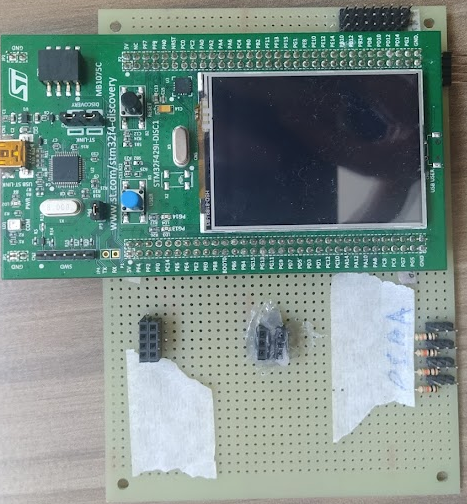
\includegraphics[width=1\textwidth]{Images/pcb2.png}
		\end{figure}

		Предна страна 
		\column{0.5\textwidth}
		\pause
		\begin{figure}[htpb!]
			\centering
			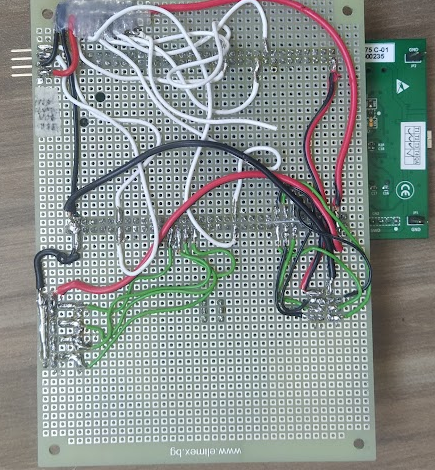
\includegraphics[width=1\textwidth]{Images/pcb1.png}
		\end{figure}

		Задна страна
	\end{columns}

\end{frame}


\begin{frame}{Подбрани портове, пинове и периферия}
	\pause
		\begin{block}{I2C}
			\pause
				PA8 (I2C3 SCL) и PA9 (I2C3 SDA). Цялата периферия по шината оперира на 3.3V.
		\end{block}
		\pause

		\begin{block}{USART}
			\pause
			PB6(USART1 TX) и PB7 (USART1 RX). Цялата периферия по шината оперира на 3.3V.
		\end{block}
		\pause

		\begin{block}{Управляващи сигнали ESC}
			\pause
			PD12 - PD15. Конфигурация Open-drain, външни Pull-up резистори \(10M\Omega\).
			Нужно е да се генерира 5V PPM сигнал.
		\end{block}

\end{frame}


\begin{frame}[t]
\pause

		\begin{block}{Входове PPM (приемник, сензор за разстояние)}
			\pause
						PA0(TIM5 канал 1), PA3(TIM5 канал 4), PB0(TIM3 канал 3),
			PB1(TIM3 канал 4), PB4(TIM3 канал 2), PB5(TIM3 канал 1).
			Периферията генерира 5V сигнали на входа. Входовете са 5V толерантни.
		\end{block}

\end{frame}

\begin{frame}{Балансиране на витла}
	\begin{columns}
		\column{0.5\textwidth}
		\pause
	\begin{figure}[htpb!]
		\centering
		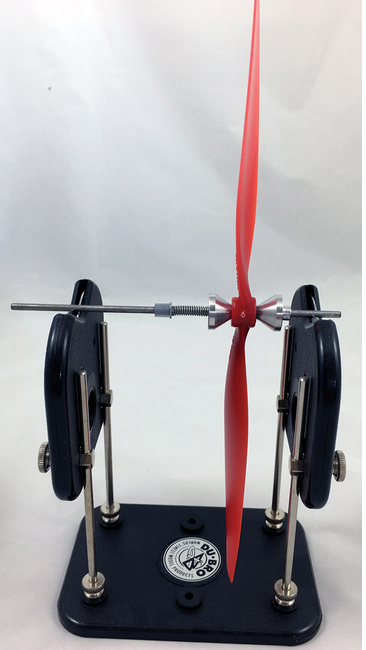
\includegraphics[width=0.5\textwidth]{Images/prop_on_balance.png}
		\caption{Небалансирано витло}
	\end{figure}


	\column{0.5\textwidth}

	\pause
		\begin{figure}[htpb!]
		\centering
		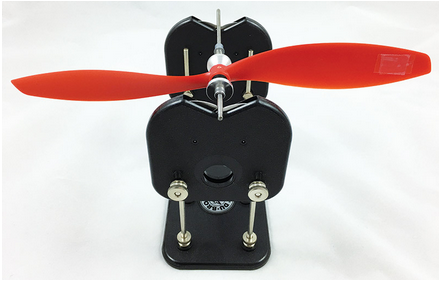
\includegraphics[width=0.85\textwidth]{Images/prop_balanced.png}
		\caption{Балансирано витло}
	\end{figure}
\end{columns}
\end{frame}

\begin{frame}{Основа за монтиране на контролер и външна периферия}
	\begin{columns}
		\column{0.5\textwidth}
		\pause
		\begin{figure}[htpb!]
		\centering
		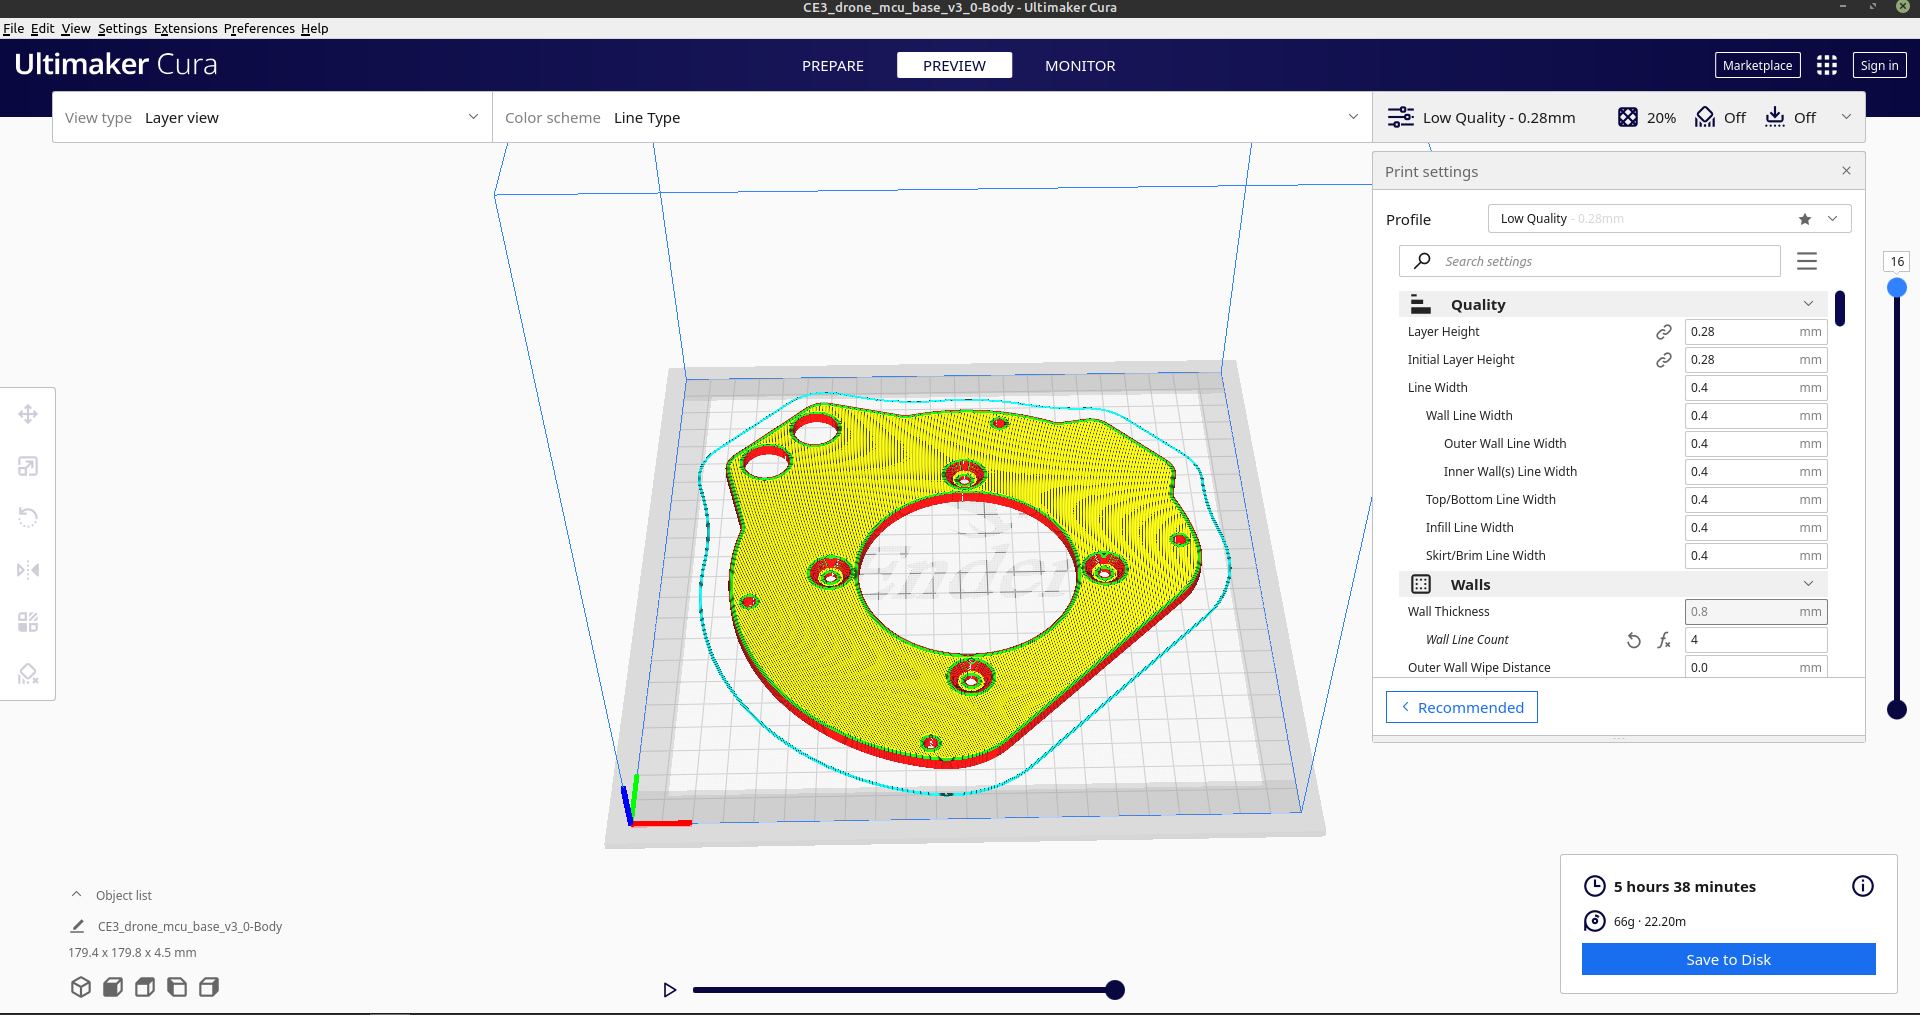
\includegraphics[width=1\textwidth]{Images/ultimaker_cura_window.png}
		\caption{Основа за монтиране, Ultimaker Cura}
	\end{figure}


	\column{0.5\textwidth}
	\pause
	\begin{figure}[htpb!]
		\centering
		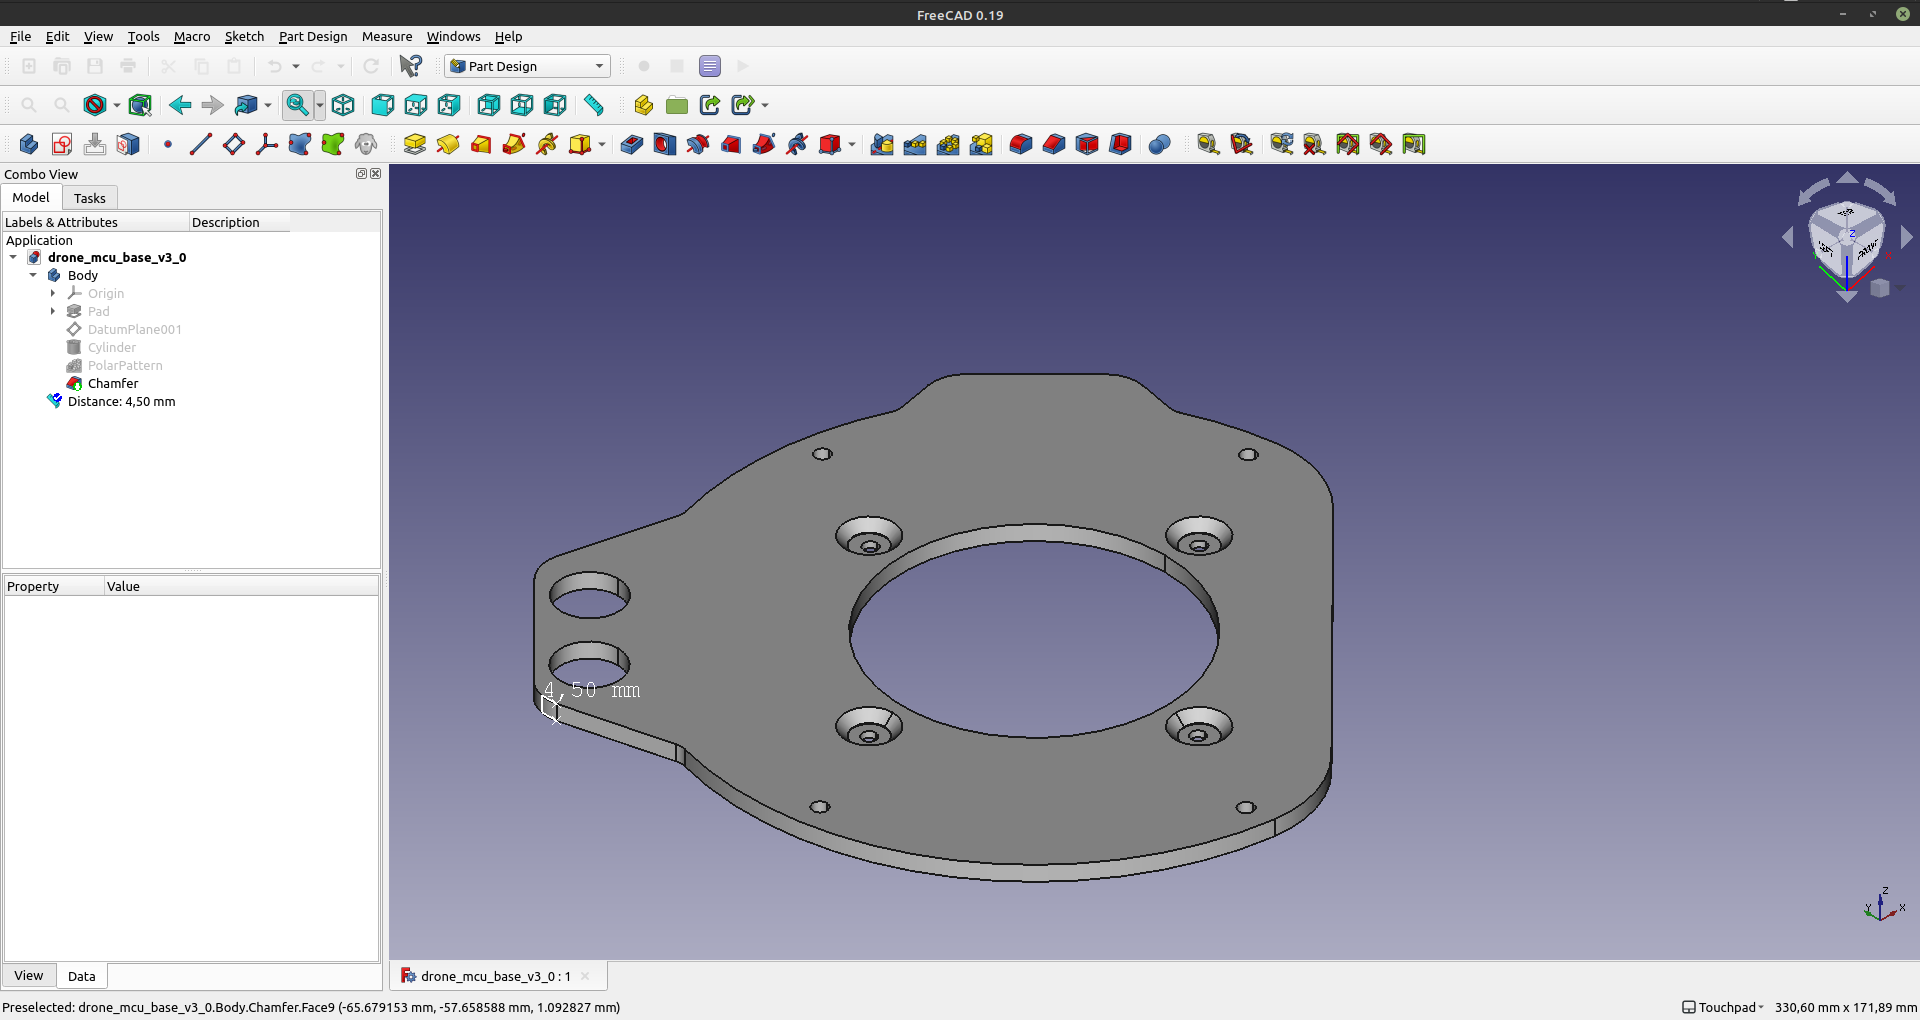
\includegraphics[width=1\textwidth]{Images/freecad_window.png}
		\caption{Основа за монтиране FreeCad}
	\end{figure}
\end{columns}

\end{frame}

\begin{frame}{Платформа за управление на \\ъгъл на завъртане}
	\pause
	\begin{figure}[htpb!]
		\centering
		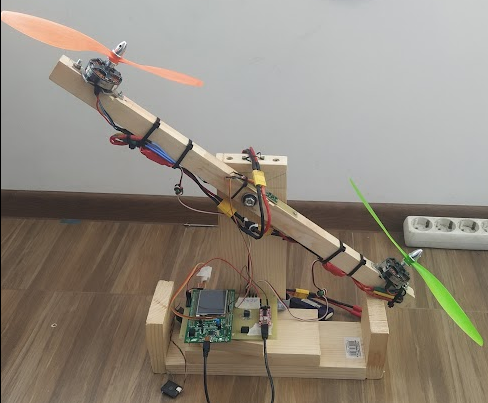
\includegraphics[width=0.6\textwidth]{Images/balance_construction.png}
	\end{figure}

\end{frame}

\begin{frame}{Платформа за безпилотен летателен апарат \\с четири ротора }
	\pause
	\begin{figure}[htpb!]
		\centering
		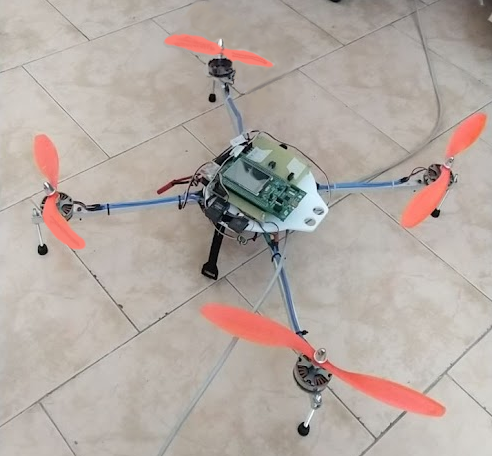
\includegraphics[width=0.6\textwidth]{Images/drone_construction.png}
	\end{figure}
\end{frame}




\section{Моделиране и \\идентификация}

\subsection{Ротор с витло}

\begin{frame}{Моделиране на ротор с витло}
	\pause
	Опростен апроксимиран модел - нискочестотен филтър и коефициент на пропорционалност.
	\pause
	\begin{figure}[htpb!]
		\centering
		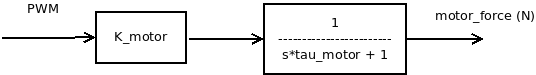
\includegraphics[width=0.7\textwidth]{Images/motor_model.png}
		\caption{Опростен модел на витло и мотор}
		\label{fig:motor_model}
	\end{figure}
	\pause
	\begin{equation*}
		G_{motor}(s) = \frac{k_{motor}}{s \tau_{motor} + 1}
		\label{eqn:motor_model}
	\end{equation*}

\end{frame}

\begin{frame}{Снемане на характеристики на \\ротор с витло}
	\pause
\begin{figure}[htpb!]
    \centering
    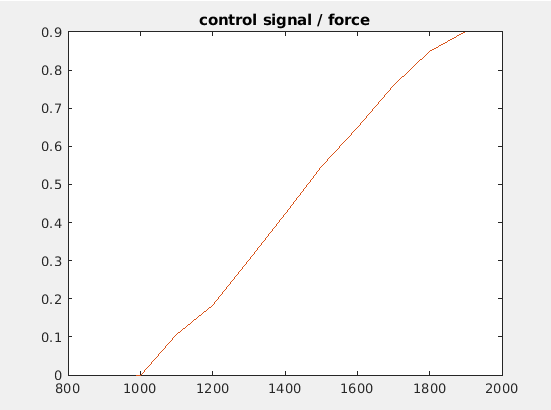
\includegraphics[width=0.6\textwidth]{Images/control_force.png}
\end{figure}

\pause
\(k_{motor} = 12.2e-3\) при сигнал \(1300\to1700\).
\pause

Опорната точка при тяга \(424g \approx 4.15N\)

\end{frame}

\subsection{Платформа за управление на ъгъл на\\ завъртане}

\begin{frame}{Моделиране на платформа за\\управление на ъгъл на завъртане}
	\begin{columns}
		\column{0.5\textwidth}

		Ако приемем:
		\begin{align*}
			F_2 &= F_0 + \delta f,F_1 &= F_0 - \delta f 
		\end{align*}
		И апроксимираме:
		\begin{align*}
			I &= \frac{l^2}{12}(M + 6m)
		\end{align*}

		Получаваме:\\[1em]

		\column{0.5\textwidth}
		
		\begin{figure}[htpb!]
			\centering
			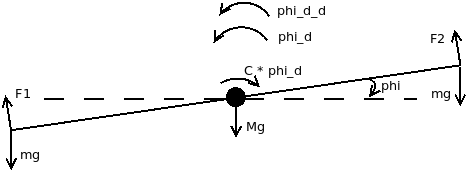
\includegraphics[width=0.9\textwidth]{Images/balance_force_diagram.png}
		\end{figure}

	\end{columns}

	\begin{equation*}
	G_{sys} = G_{motor}(s)G_{platform}(s) = 
	\frac{k_{motor} l}{s( s I + C)(s \tau_{motor} + 1)} 
	\end{equation*}

\end{frame}

\begin{frame}{Идентификация на параметри на \\ платформа за управление на ъгъл на \\завъртане}
	\pause
		След снемане на преходен процес:
		\pause
		
		\(I = 0.025, C = 0.018, \tau_{motor} = 0.08\)
		\pause

	\begin{figure}[htpb!]
		\centering
		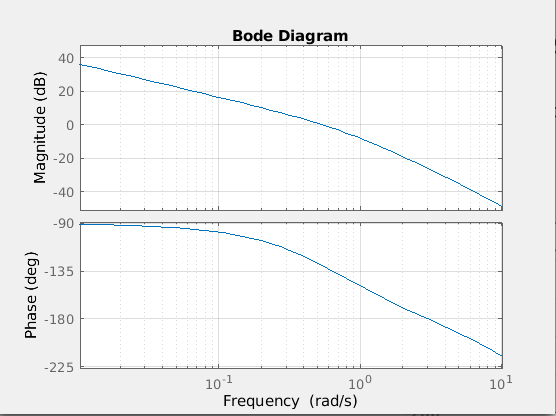
\includegraphics[width=0.5\textwidth]{Images/bode_balance.png}
	\end{figure}
\end{frame}


\subsection{Платформа за безпилотен летателен апарат с четири ротора}


\begin{frame}{Конфигурация}
	\pause
	\begin{figure}[!h]
		\centering
		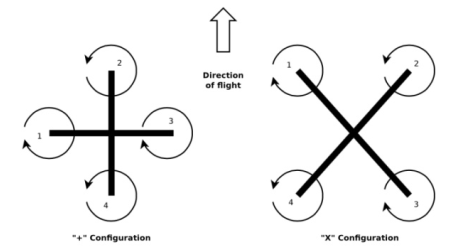
\includegraphics[width=0.9\columnwidth]{Images/rotors.png}
	\end{figure}
\end{frame}

\begin{frame}{Сили, моменти и отправни координaтни системи}
	\pause
\begin{figure}[!h]
    \centering
    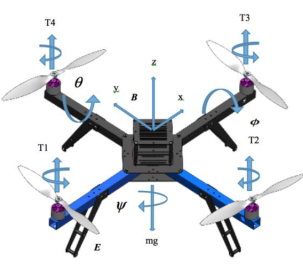
\includegraphics[width=0.6\columnwidth]{Images/kinematika.png}

\end{figure}
\end{frame}

\begin{frame}{Моделиране}
	\pause
	За да се носи платформата във въздуха, е нужно:
	\pause

\begin{align*}
		\sum_{i=1}^{4} T_i  =& -mg \\
		\sum_{i=1}^{4} M_i  =& 0 \\
		T_{1,2,3,4} ||& g \\
		( \omega_1 + \omega_3 ) - ( \omega_2 + \omega_4 ) =& 0 
\end{align*}
\pause

от което и следва, че \(\phi=0,\theta=0,\psi=0\).

\end{frame}
\begin{frame}
	\pause
		За промяна на ориентацията се налага да:
		\pause
		
		\begin{align*}
		\dot{\psi} = k_{\psi}((\omega_1+\omega_3)-(\omega_2 + \omega_4)) ,& \psi = \int \dot{\psi}dt\\
		\dot{\phi} = k_{\phi}((\omega_1 + \omega_4) - (\omega_2+\omega_3 )) ,& \phi = \int \dot{\phi}dt\\
		\dot{\theta} = k_{\theta}((\omega_1+\omega_2) - (\omega_3 +\omega_4)) ,& \theta = \int \dot{\theta}dt
\end{align*}
\end{frame}

\begin{frame}{Моделиране на системата чрез блок схема}
	\pause
	\begin{figure}[!h]
		\centering
		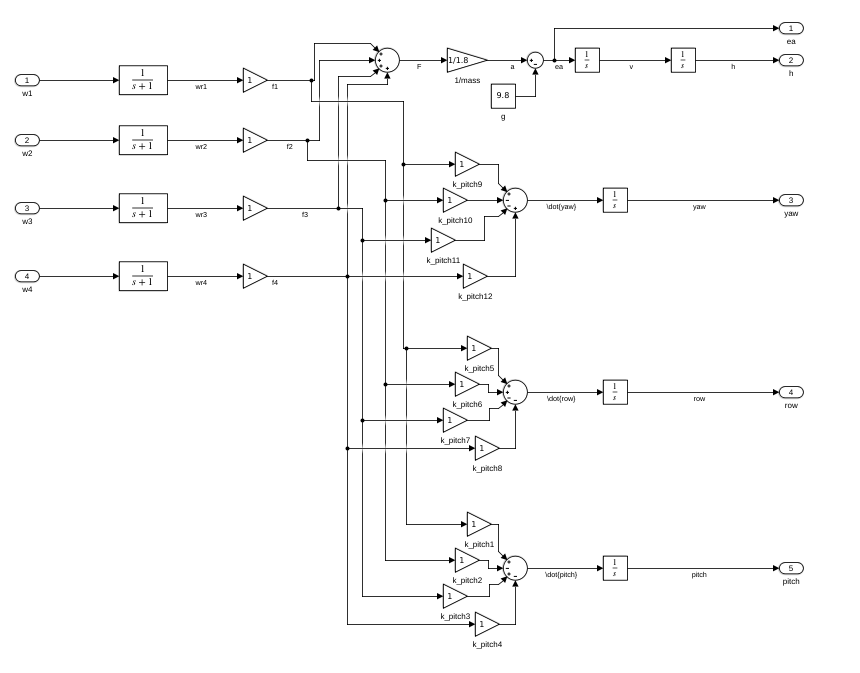
\includegraphics[width=0.7\columnwidth]{Images/quadrotor_simulink.png}
	\end{figure}
\end{frame}


\section{Калибриране и компенсация}

\subsection{Жироскопен дрейф}

\begin{frame}{Компенсация на жироскопен дрейф по\\температура}
	\pause
    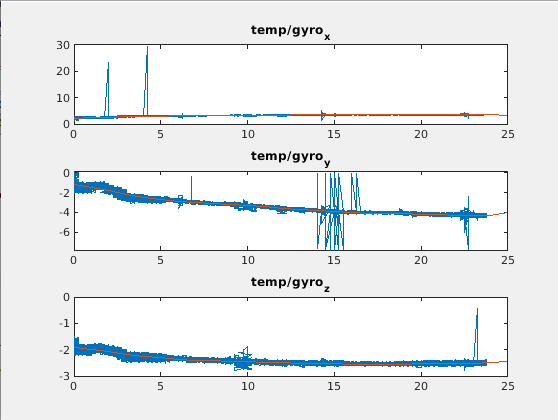
\includegraphics[width=0.8\textwidth]{Images/gyro_drift_calibrate.png}

\end{frame}

\begin{frame}[fragile]
	\pause
	\begin{verbatim}
	  p_x = 
		  -42.6978e-9  x^7 +  3.7797e-6 x^6  -131.8066e-006 x^5 + 2.2717e-3 x^4  -19.5918e-3 x^3 +  67.9744e-3 x^2 + 95.1384e-3 x + 2.2440e+0
	
	  p_y =
		  87.1716e-9 x^7  -7.6384e-6 x^6 +  263.1019e-006 x^5  -4.4660e-3 x^4 37.8030e-3 x^3  -129.2365e-3  x^2 -191.6577e-3 x -1.1695e+0
	
	  p_z =
		  15.9591e-9 x^7  -1.4613e-6  x^6 + 53.0721e-006 x^5  -961.5439e-6 x^4 +  8.8365e-3  x^3 -33.3197e-3  x^2 -44.0584e-003 x -1.9076e+0
	\end{verbatim}
	\end{frame}


\subsection{Магнитни отмествания от околната среда}

\begin{frame}{Компенсация на магнитни отмествания от околната среда}
	\pause
	\begin{figure}[!h]
		\centering
   		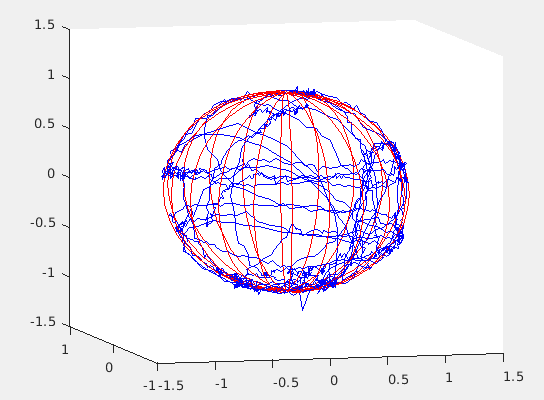
\includegraphics[width=0.6\textwidth]{Images/mag_calibration.png}
	\end{figure}
	\pause
	Използвана е техника на Мерайо\cite{merayo2000scalar} \\(трансформация отместен елипсоид - центрирана сфера).
\end{frame}


\begin{frame}[fragile]
	\pause
	\begin{verbatim}
		U =
	
		21.4229e+000   837.9000e-003     3.0861e+000
		 0.0000e+000    21.6201e+000     2.0207e+000
		 0.0000e+000     0.0000e+000    27.2441e+000
	
		c =
	
		-1.6000e-003
		19.9000e-003
		45.7000e-003
	\end{verbatim}
	\end{frame}




\section{Синтез на наблюдател}

\begin{frame}{Филтър на Калман за оценка на \\ъгъл на завъртане}
	\pause
	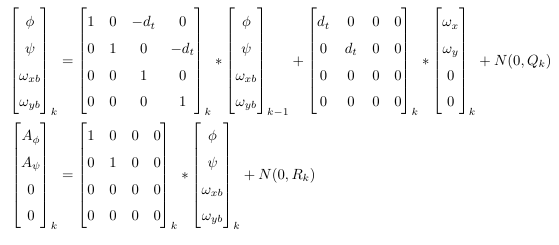
\includegraphics[width=\textwidth]{Images/kf.png}
\end{frame}


\begin{frame}{Ковариантни матрици}
	\pause
\begin{align*}
    Q =
    \begin{bmatrix}
        33.8 & 0 & 0 & 0 \\
        0 & 33.8 & 0 & 0 \\
        0 & 0 & 0.4 & 0 \\
        0 & 0 & 0 & 0.4
    \end{bmatrix} &,&
    R = \begin{bmatrix}
        32 & 0 & 0 & 0 \\
        0 & 32 & 0 & 0 \\
        0 & 0 & 0 & 0 \\
        0 & 0 & 0 & 0
    \end{bmatrix}
\end{align*}
\end{frame}

\begin{frame}{Проверка на резултатите}
	\begin{columns}
		\column{0.5\textwidth}
		\pause
				\begin{figure}[htpb!]
			\centering
			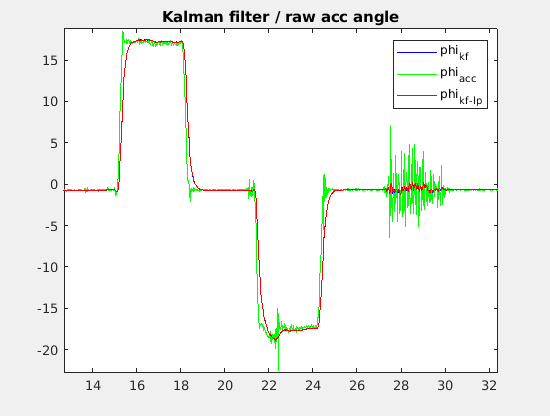
\includegraphics[width=\textwidth]{Images/kalman_filter_time_vs_raw.png}

		\end{figure}
		

		\column{0.5\textwidth}
		\pause
		\begin{figure}[htpb!]
			\centering
			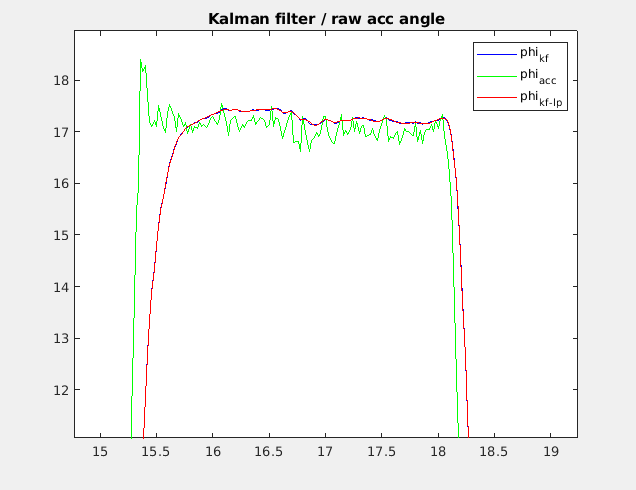
\includegraphics[width=\textwidth]{Images/kalman_filter_time_vs_raw_2.png}

		\end{figure}
	\end{columns}
\end{frame}

\section{Синтез на управление}

\begin{frame}{Управление на ъгъл на завъртане}
	\pause
	Опростена схема на управлението: 
	\begin{figure}[htpb!]
		\centering
		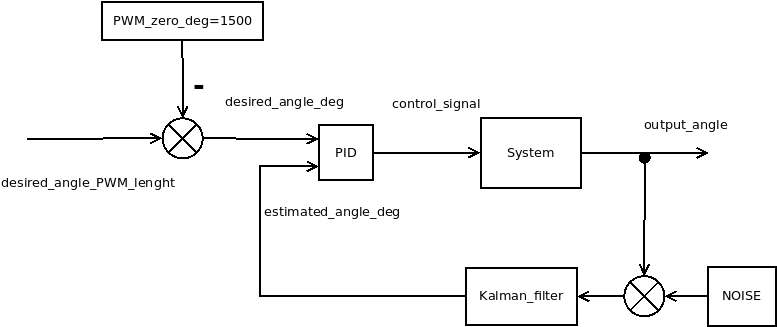
\includegraphics[width=1\textwidth]{Images/control_diagram_simple.png}
	\end{figure}
\end{frame}

\begin{frame}{Схема на имплементирания универсален ПИД}
	\pause

	\begin{figure}[htpb!]
		\centering
		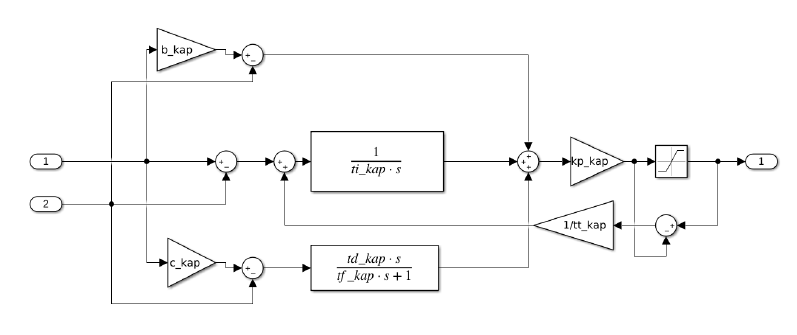
\includegraphics[width=1\textwidth]{Images/universal_pid.png}
	\end{figure}

\end{frame}

\begin{frame}{Параметри на регулатор и преходен процес}
	\pause
	\begin{equation*}
		K_p=0.4, K_i=0.003, K_d=2, \tau_d=0.26, out_{limit}=\pm150
	\end{equation*}
	\pause
	\begin{figure}[htpb!]
		\centering
		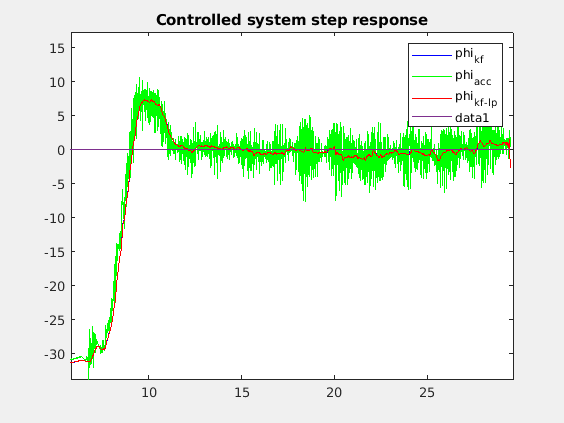
\includegraphics[width=0.7\textwidth]{Images/controlled_system.png}
	\end{figure}
\end{frame}


%\begin{frame}[focus]
%	Тази презентация е създадена с помощта на \textit{beamer} \LaTeX \textit{- Focus}
%\end{frame}

%\begin{frame}[focus]
%	Специялни благодарности на \textit{Кристина Дойчева} за редакция и офрмление.
%\end{frame}


%----------------------------------------------------------------------------------------
%	 CLOSING/SUPPLEMENTARY SLIDES
%----------------------------------------------------------------------------------------

\begin{frame}[focus]
	Предложения за надграждане.
\end{frame}

\begin{frame}[focus]
	Заключение.
\end{frame}

\begin{frame}{Литература}
	\nocite{*} % Display all references regardless of if they were cited
	\bibliography{example.bib}
	\bibliographystyle{plain}
\end{frame}

%------------------------------------------------

\begin{frame}[focus]
	Благодаря за вниманието!
\end{frame}


%----------------------------------------------------------------------------------------

\end{document}
